\documentclass{ctexart}
\usepackage[a4paper,top=3cm,bottom=2.7cm,left=2.54cm,right=2.54cm]{geometry}
\usepackage{amsmath,amsfonts,amssymb,amsthm}
\usepackage{graphics}
\usepackage{tikz}
\usepackage{multirow}
\usepackage{array}
\usepackage{fancyhdr}
\usepackage{lastpage}
\usepackage{indentfirst}
\usepackage{draftwatermark}         % 所有页加水印
%\usepackage[firstpage]{draftwatermark} % 只有第一页加水印
\SetWatermarkText{数字电路-期中-模拟}           % 设置水印内容
%\SetWatermarkText{\includegraphics{fig/texlion.png}}         % 设置水印logo
\SetWatermarkLightness{0.8}             % 设置水印透明度 0-1
\SetWatermarkScale{0.3}   
\pagestyle{fancy}
\fancyhf{}
\cfoot{第 \thepage 页 \quad 共 6 页}
\rhead{2023—2024 学年第一学期\quad }
\lhead{命题:Z \qquad 验题:W}
\renewcommand{\headrulewidth}{0.7pt}
%\renewcommand{\labelenumi}{\Arabic{enumi}}

\begin{document}

\vspace{1em}
\begin{center}

\textbf{\LARGE NJUIC 《 数字电路 》期中模拟考试试卷}
\end{center}

\begin{center}
\begin{tabular}{m{0.3\textwidth} m{0.3\textwidth} m{0.3\textwidth}}
     
     考试时长:120分钟 & 考生学号:&考生姓名:
\end{tabular}
\end{center}
\vspace{-0.3cm}
\hrule height 0.5pt
%\noindent
%\rule{\textwidth}{1pt}

\subsection*{一、(29 分)填空题}
\subsubsection*{1. 请帮Z同学完成下列简单填空(每空1分,共16分)}
\vspace{-0.2cm}
(1) 请将十六进制数$(79)_{16}$转换为十进制数(\qquad \qquad ).\par
(2) 请将十进制数2024转换为十六进制数(\qquad \qquad ).将二进制数11011001.01B转换为八进制数(\qquad \qquad ).\par
(3) 将十进制数23转换为二进制数(\qquad \qquad  ).\par
(4) 将十进制数3.375转换为二进制数(\qquad \qquad ).\par
(5) 四位有符号数A=$(1101)_2$,A的1的补码是(\qquad \qquad  ),2的补码是(\qquad \qquad  ).\par
(6) 2024个“1”连续进行异或运算,其结果是(  \qquad \qquad    ).\par
(7) CMOS异或门有两个输入端A和B,要实现$Y=\overline{X}$最好将输入端B(\qquad \qquad  ).\par
(8) 实现两个一位二进制数相加,产生一位和值及一位进位值,考虑低位来的进位的加法器称为(\qquad \qquad  ).\par
(9) 若一种门电路的抗干扰能力强,则其噪声容限(\qquad \qquad  ).\par
(10) 为什么不宜将多个二极管门电路串联起来使用?首先:二极管门电路的输出的高低电平数值和输入的高低电平数值不相等,相差一个(\qquad \qquad  ) .\par
(11) 在CMOS集成电路中,以金属-氧化物-半导体场效应晶体管(Metal Oxide Semico- nductor Field Effect Transistor, 简称MOS管)作为开关器件.在P型半导体衬底上,制作两个高掺杂浓度的N型区,形成MOS管的(\qquad \qquad  ) 和漏极.第三个电极称为  (\qquad \qquad  )  ,通常用金属铝或多晶硅制作.\par
(12) CMOS电路的动态功耗和哪些电路参数有关? 请给出其中两个参数  (\qquad \qquad  )  、 (\qquad \qquad  ).\par

\subsubsection*{2.Z同学面临化简以下逻辑函数的难题,请帮助解决(5 分)}
\vspace{-0.2cm}
(1) $Z(A,B,C)=\Sigma m(0,1,2,5,6,7)$\par
\vspace{0.8cm}
(2) $Z(A,B,C,D,E,F,G)=AB+A\overline{C}+\overline{B}C+ADE(F+G)+B\overline{D}+\overline{C}\, \overline{D}$
\vspace{0.8cm}

\subsection*{3. 数字芯片设计包含多个过程,请帮助Z同学写出以下图文中逻辑函数 (每空 2 分)}
\vspace{-0.1cm}
(1) $f=$\par
\begin{figure}[htbp]
    \centering
    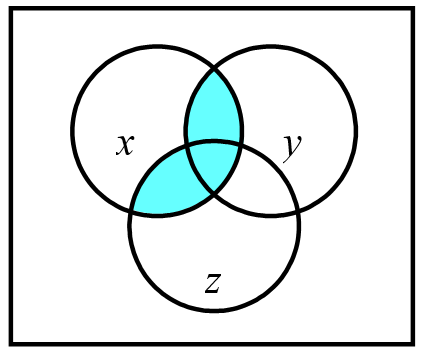
\includegraphics[width=0.28\linewidth]{1.png}
\end{figure}
(2) $L=$\par
\begin{figure}[htbp]
    \centering
    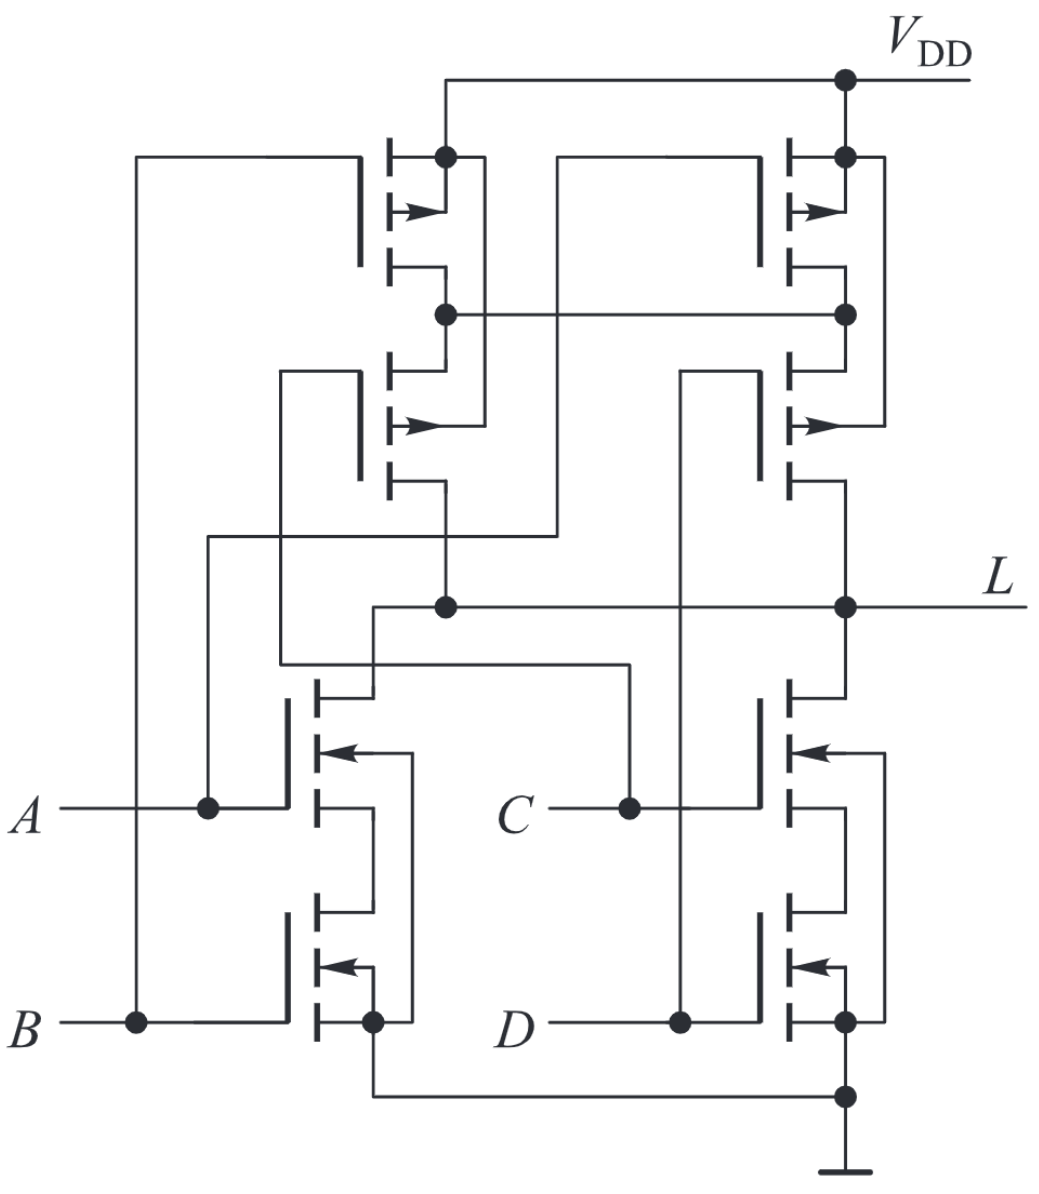
\includegraphics[width=0.35\linewidth]{2.png}
\end{figure}
(3) $f=$\par
\begin{figure}[htbp]
    \centering
    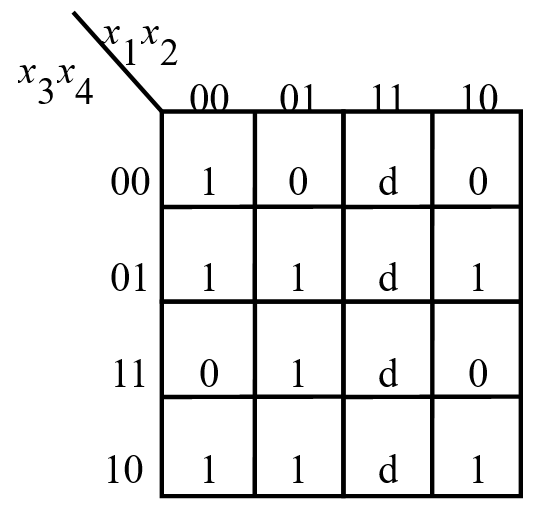
\includegraphics[width=0.3\linewidth]{3.png}
\end{figure}
(4) $f=$\par

    \qquad \textbf{module function (w0, w1, w2, w3, S, f);}\par
    \qquad \qquad \textbf{input w0, w1, w2, w3;}\par
    \qquad \qquad \textbf{input [1:0] S;}\par
    \qquad \qquad \textbf{output f;}\par
    \qquad \qquad \textbf{assign f = S[1] ? (S[0] ? w3 : w2) : (S[0] ? w1 : w0);}		\par
    \qquad \textbf{endmodule }

\subsection*{二、(8分)}
Z同学被要求只用“与非”门实现函数$f(x_1,x_2,x_3)= \Sigma m(2,4,6,7)$的功能.请先推导该函数的SOP表达式,并帮助Z同学画出电路图.
\newpage
\subsection*{三、(8分)}
Verilog代码描述了硬件的逻辑结构,Z同学设计电路时书写了以下代码.\par

{\small
\qquad \textbf{module problem3 (IN, OUT);}\par
   \qquad \qquad \textbf{input [3:0] IN;}\par
   \qquad \qquad \textbf{output reg [3:0] OUT;}\par
\qquad    \qquad \textbf{always @(IN) begin}\par
\qquad    \qquad \qquad      \textbf{if (IN==4'b0001)   OUT<=4'b0001;}\par
\qquad    \qquad \qquad      \textbf{else if (IN==4'b0010) OUT<=4'b0010;}\par
\qquad    \qquad \qquad      \textbf{else if (IN==4'b0011) OUT<=4'b0011;}\par
\qquad    \qquad \qquad      \textbf{else if (IN==4'b0101) OUT<=4'b0010;}\par
\qquad    \qquad \qquad      \textbf{else if (IN==4'b0110) OUT<=4'b0100;}\par
\qquad    \qquad \qquad      \textbf{else if (IN==4'b0111) OUT<=4'b0110;}\par
\qquad    \qquad \qquad      \textbf{else if (IN==4'b1001) OUT<=4'b0011;}\par
\qquad    \qquad \qquad      \textbf{else if (IN==4'b1010) OUT<=4'b0110;}\par
\qquad    \qquad \qquad      \textbf{else if (IN==4'b1011) OUT<=4'b1001;}\par
\qquad    \qquad \qquad      \textbf{else if (IN==4'b1101) OUT<=4'b0100;}\par
\qquad    \qquad \qquad      \textbf{else if (IN==4'b1110) OUT<=4'b1000;}\par
\qquad     \qquad \qquad     \textbf{else if (IN==4'b1111) OUT<=4'b1100;}\par
\qquad    \qquad \qquad      \textbf{else OUT=4'b0000;}\par
\qquad  \qquad \textbf{end} \par
\qquad     \textbf{endmodule}\par
}
(1)帮助Z同学给出信号IN和OUT之间的关系. \par
(2)评价Z同学书写的代码是否为其描述的功能提供了一种好的实现风格,请分析.
\vspace{4.2cm}

\subsection*{四、(8分)}
Z同学知道香农展开对于逻辑条件的梳理很有作用,请对函数$f(w_1,w_2,w_3)=\Sigma m(0,2,6,7)$采用香农展开. 请用一个2选1多路选择器和其他必要的门电路实现此函数,再请用一个4选1多路选择器和其他必要的门电路实现此函数.

\newpage
\subsection*{五、(8分)}
请利用卡诺图帮助Z同学求函数 $f(x_1,x_2,x_3,x_4) = \Sigma m (4,6,8, 10 , 11 ,12,14)$ 的最低成本SOP表达式. 假定无关项为$D=\Sigma m(3,5,7,9,15)$.\par
\vspace{4cm}

\subsection*{六、(12分)}
在计算机运算中常常要比较数字的大小,Z同学对加法器的构造做修改得到一减法器如下图,可实现两4位有符号数$X=x_3x_2x_1x_0$、$Y=y_3y_2y_1y_0$减法$X-Y$. 3个输出结果的意义如下:\par
(1)结果是0,Z = 1,否则 Z = 0 ;\par
(2)结果是负数,N = 1,否则 N = 0 ;\par
(3)如果发生算术溢出 V = 1,否则 V = 0 .\par
请说明如何利用Z、N和V判断$X=Y$, $X<Y$, $X>Y$.如果$X,Y$仅是二进制数(无符号数),该电路该做如何修改并判断呢?\par
\vspace{-0.3cm}
\begin{figure}[htbp]
    \centering
    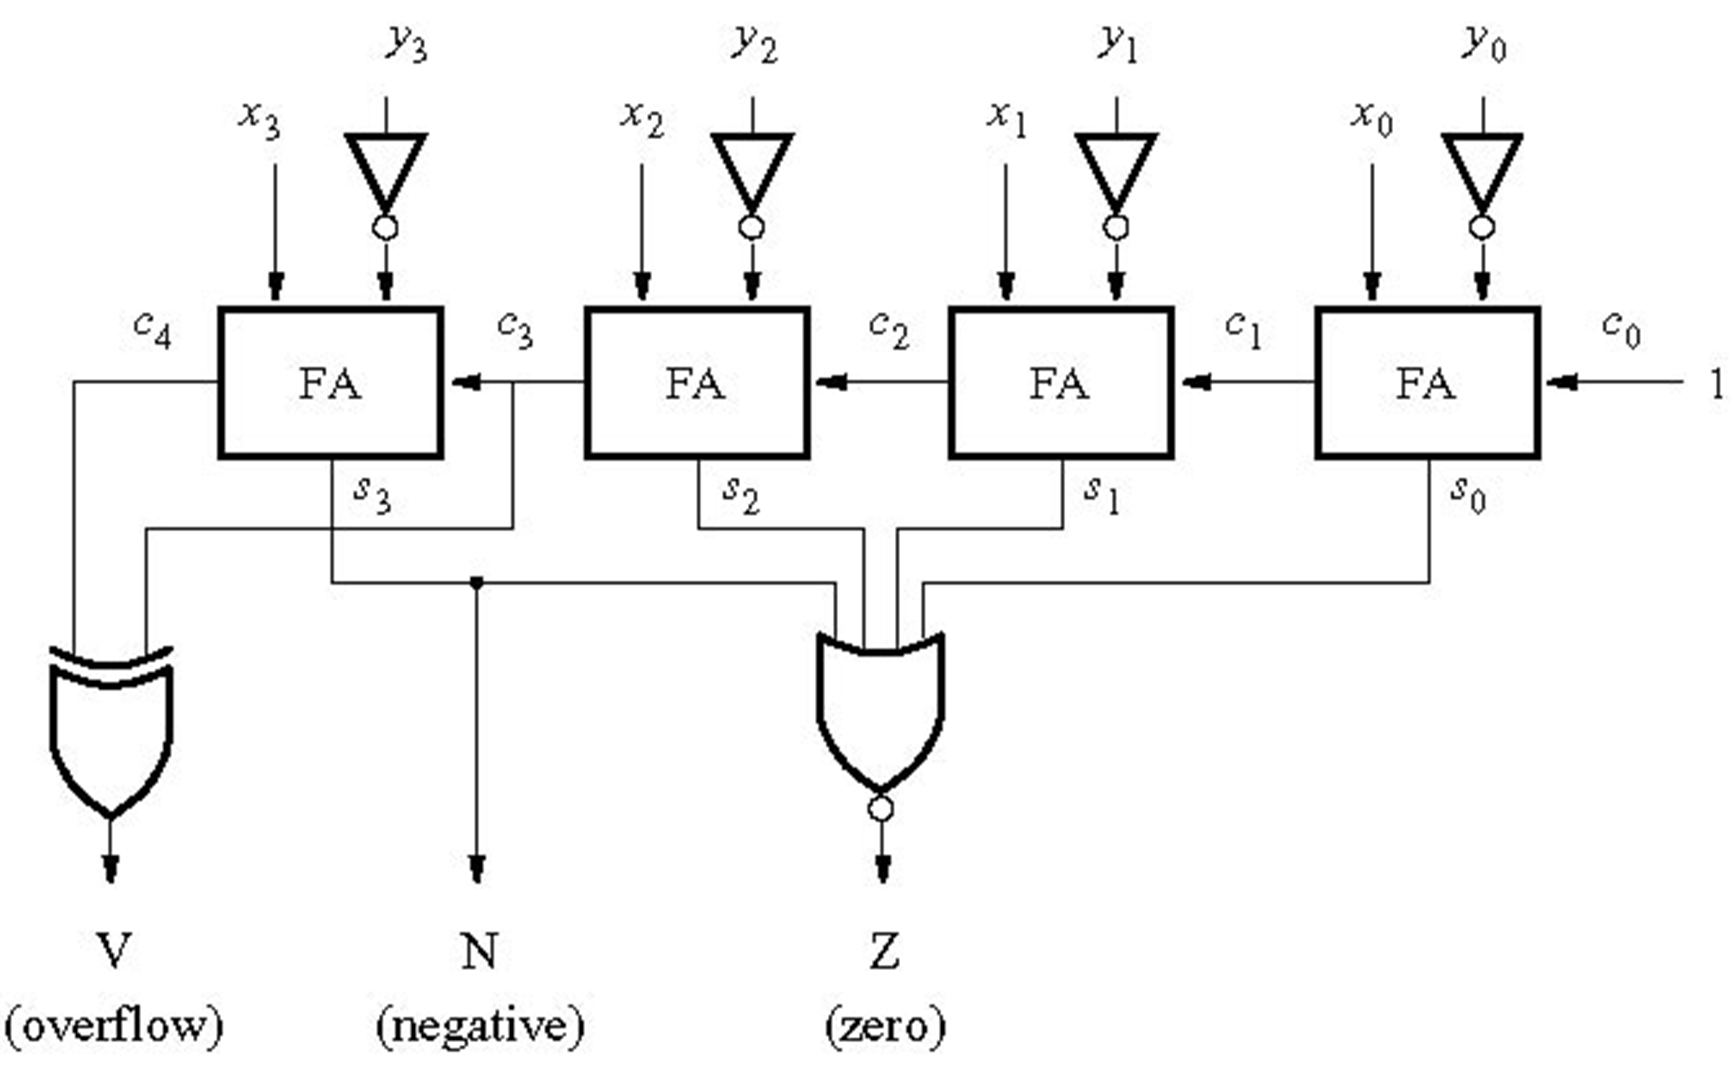
\includegraphics[width=0.7\linewidth]{4.png}
\end{figure}

\newpage
\subsection*{七、(12分)}
Z同学需要构建一数字电路,其输入为三位二进制数$X=x_2x_1x_0$,输出为五位二进制数$Y=y_4y_3y_2y_1y_0$,电路实现的功能是$Y=3X+5$.帮助Z同学完成以下内容.\par
(1)列出电路的真值表.\par
(2)写出输出$y_2$的标准SOP表达式,并用3-8译码器实现.\par
(3)写出输出$y_i$的最简SOP表达式.
\vspace{8cm}

\subsection*{八、(8分)}
Z同学希望仅用加法电路与2选1数据选择器设计一个电路,以实现用1, 3, 4, 6乘以一个8位二进制数字$A=a_7,...,a_0$,分别产生结果$A$、$3A$、$4A$或者$6A$. 请帮助Z同学给出设计思路并画出简要电路图.

\newpage

\subsection*{九、(8分)}
现场可编程门阵列(FPGA)中包含了用于实现逻辑函数的查找表(LUT).每个LUT可以通过编程实现任何输入的逻辑函数,很多商用FPGA包含4输入的查找表单元.请用多个4输入查找表来构建一个选择输入信号为$S_1$、$S_0$和数据输入信号$w_3$、$w_2$、$w_1$、$w_0$的4选1多路选择器.\par
2.	请通过表达式变换,用3个LUT实现4选1多路选择器并画出框图.\par
3.	继续变换表达式,用2个LUT实现4选1多路选择器并画出框图.


\end{document}
